\documentclass[a4paper]{report}
\usepackage[utf8]{inputenc}
\usepackage[T1]{fontenc}
\title{Relatório - Python vs. Java}
\author{Ana Almeida e Pedro Alagoa}
\date{Fevereiro 2014, Universidade de Aveiro}
\usepackage[portuguese]{babel}
\usepackage{indentfirst}
\usepackage[colorlinks=true,
            linkcolor=blue,
            urlcolor=blue,
            citecolor=red]{hyperref}
\usepackage{graphicx}
\usepackage{url}
\usepackage{glossaries}

\usepackage[procname]{listings}
\usepackage{color}

\definecolor{dkgreen}{rgb}{0,0.6,0}
\definecolor{gray}{rgb}{0.5,0.5,0.5}
\definecolor{mauve}{rgb}{0.58,0,0.82}

\definecolor{keywords}{RGB}{255,0,90}
\definecolor{comments}{RGB}{0,0,113}
\definecolor{red}{RGB}{160,0,0}
\definecolor{green}{RGB}{0,150,0}
 
\lstset{language=Python, 
        basicstyle=\ttfamily\small, 
        keywordstyle=\color{keywords},
        commentstyle=\color{comments},
        stringstyle=\color{red},
        showstringspaces=false,
        identifierstyle=\color{green},
        }
        
% Glossário
\makeglossaries
\usepackage{glossaries}

\newglossaryentry{Explicit is better than implicit}{name=Explicit is better than implicit :, description={Explícito é melhor que implícito.}}
\newglossaryentry{Beautiful is better than ugly}{name=Beautiful is better than ugly :, description={Bonito é melhor que feio.}}
\newglossaryentry{Simple is better than complex}{name=Simple is better than complex :, description={Simples é melhor que complexo.}}
\newglossaryentry{Readability counts}{name=Readability counts :, description={A legibilidade conta.}}

\bibliographystyle{unsrt}

\addcontentsline{toc}{section}{References}


\begin{document}
\begin{flushleft}
\begin{center}
 \Large{Universidade de Aveiro}
 \\[150pt]
 \fbox {\huge{Python vs. Java}}
 \\[75pt]
 \flushright{Ana Almeida}
 \\
 \flushright{Pedro Alagoa}
 \\[200pt]
 \flushleft \Large Relatório no âmbito de Laboratórios de Informática
 \\
 \flushright{Fevereiro, 2014}
 \\
 Aveiro
\end{center} 

\maketitle

\begingroup
\hypersetup{linkcolor=black}
\tableofcontents
\endgroup
\clearpage

\cleardoublepage
\addcontentsline{toc}{section}{\listtablename}
\begingroup
\hypersetup{linkcolor=black}


\cleardoublepage
\addcontentsline{toc}{section}{\listfigurename}
\listoffigures
\endgroup

\clearpage

\end{flushleft}

\section{Resumo}
\label{resumo}

No seguimento da matéria que tem vindo a ser leccionada nas aulas de Laboratórios de Informática, nomeadamente Python, e com o intuito de explorar as potencialidades desta linguagem de programação, em especial quando comparada a outras linguagens de programação, como o Java, foi proposta a resolução de um guião de Programação contituído por sete exercícios que deveriam ser resolvidos nas duas linguagens e posteriormente comparar as implementações. 
\\
Os códigos escritos quer em Python quer em Java foram comparados a vários níveis, como funções, sintaxe e identação, sempre no sentido de avaliar qual a linguagem mais simples para realizar determinada instrução. Os códigos dos exercícios e as conclusões retiradas são apresentados mais detalhadamente no capítulo Análise de Resultados. 
\\
Após estabelecidas as comparações concluiu-se que Python é, no geral, uma linguagem mais simples de aprender, principalmente do ponto de vista de principiantes, pois é uma linguagem mais explícita, intuitiva, com um código mais legível e que que se assemelha mais à linguagem corrente do dia a dia do que o Java.


\chapter{Introdução}
\label{introducao}

Este relatório tem como objectivo principal dar a conhecer melhor as funcionalidades da liguagem Python. Para isso, foram realizados os exercícios do Guião 1 de Programação 2, utilizando-se Python e também Java, de modo a servir de comparação. O 'Zen of Python' deve servir como base na comparação destas duas implementações.
\\
Trata-se de um tema importante, pois permite saber de uma forma mais detalhada quais são os aspectos mais vantajosos e também os mais incovenientes quando implementamos Python.
\\
Realizaram-se 7 exercícios com cada liguagem de programação e foram comparados os seus códigos, tendo em conta aspectos como as suas funções, sintaxe e indentação.
\\
Por fim, este relatório conclui com um comentário final aos resultados obtidos após a sua análise.

\chapter{Preparação}
\label{preparacao}

\section{Máquina e sistema operativo utilizados}
\label{machines}
Os exercícios foram resolvidos em dois computadores portáteis distintos.
\\As máquinas utilizadas foram o Toshiba Satellite P50-A-125 e o Toshiba Satellite A200-2C5.
\\Os sistemas operativos utilizados foram o Windows 8 64 bit e o Windows 7 64 bit, respectivamente.

\section{Instalação das aplicações necessárias}
\label{instalaraplicacoes}

\begin{itemize}
 \item Python\cite{Python} v2.7.6 
\includegraphics[width=0.03\linewidth]{python_logo.png}
 \item JDK\cite{JDK} 6 Update 35 
\includegraphics[width=0.03\linewidth]{java_logo.png}
 \item Notepad ++ 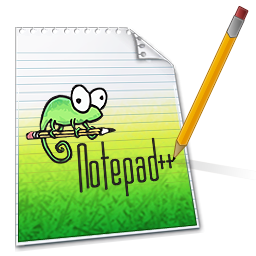
\includegraphics[width=0.03\linewidth]{notepad++_logo.png}
 \item Geany 
\includegraphics[width=0.03\linewidth]{geany_logo.png}
\end{itemize}

O \textit{download} dos programas foi realizado através dos respectivos sites oficiais.

\clearpage

\chapter{Procedimento}
\label{procedimento}

Depois de instalados e configurados os programas, procedeu-se à resolução dos exercícios do guião. O editor de texto utilizado para Java foi o Geany e o utilizado para Python foi o Notepad++.
\\
Antes dos exercícios serem resolvidos com a liguagem Python, foram revistas as regras do 'Zen of Python'. Esta lista, que é como um código de conduta para quando estamos a utilizar esta liguagem, pode ser acedida ao importar o módulo 'this', na consola do Python.
\\
Também foram revistos conceitos básicos de Python, tendo como base o Guião 12\cite{Guide12} de LABI.


\begin{figure}[ht]
 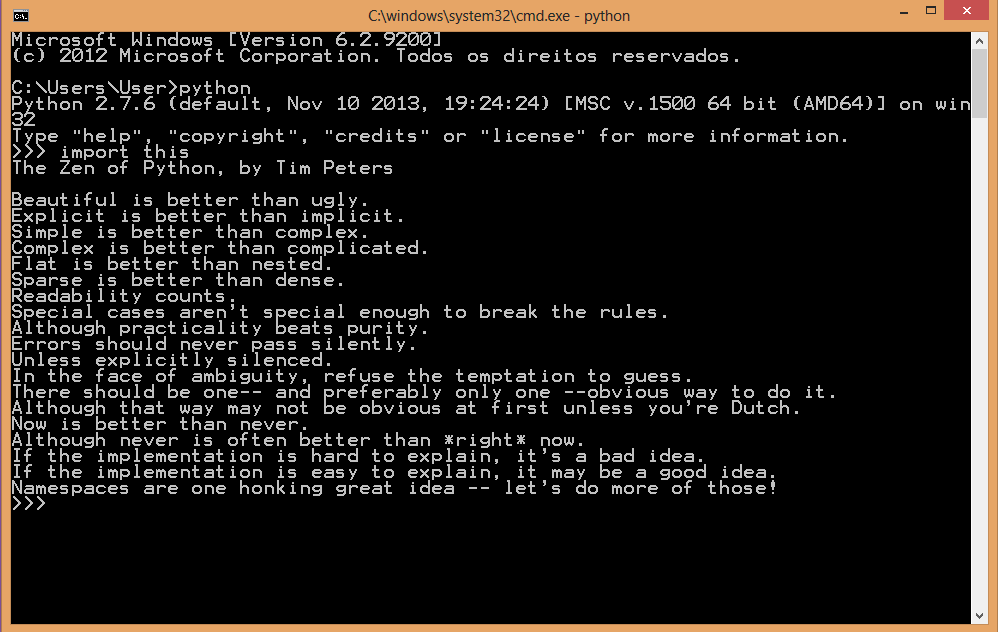
\includegraphics[width=\textwidth]{Zen_of_python.png}
 \caption{Zen of Python}
 \label{zen}
\end{figure}

Ao longo deste relatório, vamos aprofundar algumas destas regras, principalmente quando compararmos Python a Java.


\chapter{Análise de Resultados}
\label{analise}

\section{Exercício 1}
\label{exercicio1}

Crie uma calculadora simples que leia (do dispositivo de entrada) operações matemáticas como\\
12.3 + 7.2\\
e escreva o resultado respectivo (19.5 neste exemplo).\\
As operações serão sempre do género 'número' 'operador' 'número' com as três partes separadas por espaços ou em linhas diferentes. 
Implemente as quatro operações básicas. 
\\ Note que o operador é uma palavra (string) que contém apenas um símbolo.
Se for introduzido um operador inválido, deve escrever uma
mensagem apropriada para o dispositivo de saída de erros (System.err).

\begin{figure}[ht]
 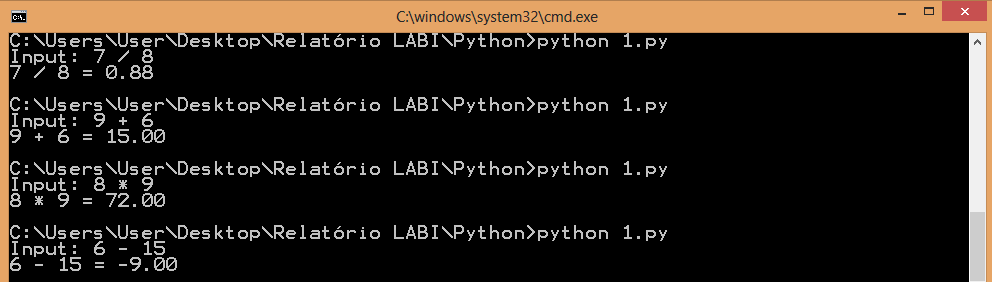
\includegraphics[width=\textwidth]{cmd_1.png}
 \caption{Execução do Exercício 1}
 \label{cmd1}
\end{figure}


O código de Java pode ser consultdo na \autoref{java.1} e o código de Python na \autoref{python.1}.

Neste exercício podemos observar um grande contraste entre Java e Python.\\
Ao contrário do Java, em que é necessário importar classes quando se pretende utilizar scanners, ler variáveis do terminal, em Python,  não implica a importação de módulos.
    \begin{description}
        \item \textbf{Java} - \fbox{import java.util.Scanner; Scanner faug = new Scanner(System.in);}
        \item \textbf{Python} - Não é necessário importar módulos nem criar scanners.
    \end{description}
\clearpage
A declaração de variáveis é bastante mais simples em Python.
    \begin{description}
        \item \textbf{Java} - \fbox{String conta = new String();conta=faug.nexLine();}
        \item \textbf{Python} - \fbox{line = raw\_input("Input: ")}
    \end{description}
Na maior parte das liguagens de programação existe o tipo 'char'. Em Python, isso não acontece, existindo apenas strings.  Isto segue a máxima "Special cases aren’t special enough to break the rules", isto é, casos especiais não são especiais o suficiente para quebrar as regras.
\\[5pt]
Na maioria das liguagens de programação, existe a funcionalidade 'switch', para quando queremos testar vários valores para uma variável. Em Python, esta funcionalidade não existe. Em detrimento do 'switch', o Python oferece Dicionários.

    \begin{description}
        \item \textbf{Java} - \fbox{switch(op) \{ case '+' ... \}}
        \item \textbf{Python} - \fbox{d = \{'+': ... \} }
    \end{description}

Aliado ao dicionário está a funcionalidade 'lambda', do Python. O comando lambda é usado para criar novos objetos função e retorná-los em tempo de execução. É uma das funcionalidades mais úteis que o Python pode oferecer.

\clearpage

\section{Exercício 2}
\label{exercicio2}

Escreva um programa que determine a nota na época normal de um aluno de Programação 2 (2013 / 2014) e que indique se o aluno está aprovado ou reprovado. Para esse fim o programa deve pedir as 4 notas necessárias (AITP1 , AIP, AITP2 ) e APF ), calcular e apresentar a nota final.


\begin{figure}[ht]
 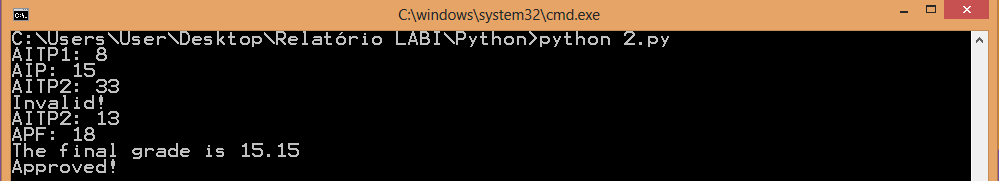
\includegraphics[width=\textwidth]{cmd_2.png}
 \caption{Execução do Exercício 2}
 \label{cmd2}
\end{figure}


O código de Java pode ser consultdo na \autoref{java.2} e o código de Python na \autoref{python.2}.

Este exercício é baseado em ciclos de repetição e lógica condicional.
Podemos observar que a maneira de representar 'ou' e 'e' são diferentes nas duas linguagens.

    \begin{description}
        \item \textbf{Java} - '||' e '\&\&'
        \item \textbf{Python} - 'or' e 'and'
    \end{description}
    
A regra "\gls{Explicit is better than implicit}" está presente neste aspecto, apesar de também se referir a situações como esta:
\\[5pt]
Implícito:
\begin{lstlisting}
from os import *
print getcwd()
}
\end{lstlisting}
vs.
Explícito
\begin{lstlisting}
import os
print os.getcwd()
}
\end{lstlisting}
\clearpage

\section{Exercício 3}
\label{exercicio3}

Escreva um programa que indique se um número (inteiro positivo) é primo.

\begin{figure}[ht]
 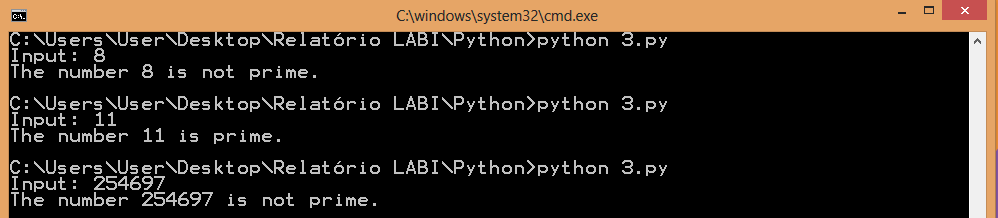
\includegraphics[width=\textwidth]{cmd_3.png}
 \caption{Execução do Exercício 3}
 \label{cmd3}
\end{figure}


O código de Java pode ser consultdo na \autoref{java.3} e o código de Python na \autoref{python.3}.

Neste exemplo é possível verificar que o código em  Python é muito mais limpo e legível.
Isto deve-se aou facto de não ser neccessária a escrita de símbolos como '\{' e ';'.
\\
Apesar de estar presente em todos os exercícios, aqui a máxima "\gls{Beautiful is better than ugly}." é bastante evidente, bem como a regra "\gls{Readability counts}."

\clearpage

\section{Exercício 4}
\label{exercicio4}

Na terra do Alberto Alexandre (localmente conhecido por Auexande Aubeto), o dialecto local é semelhante ao português com duas excepçõees:

\begin{itemize}
\item Não dizem os Rs;
\item Trocam os Ls por Us.
\end{itemize}


Implemente um tradutor de português para o dialecto do Alberto. Por exemplo “lar doce lar” deve ser traduzido para “ua doce ua”. A tradução deve ser feita linha a linha, até que surja uma linha vazia.


\begin{figure}[ht]
 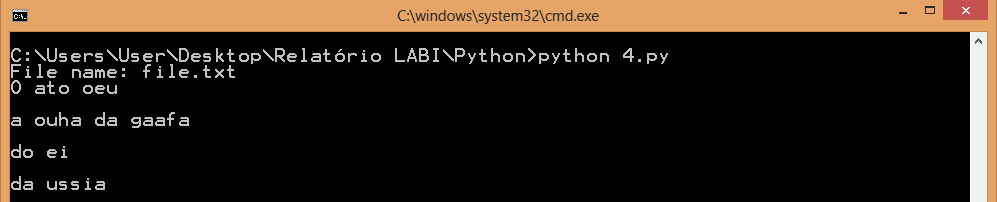
\includegraphics[width=\textwidth]{cmd_4.png}
 \caption{Execução do Exercício 4}
 \label{cmd4}
\end{figure}


O código de Java pode ser consultdo na \autoref{java.4} e o código de Python na \autoref{python.4}.

Este exercício é o melhor exemplo em termos da extensão do código.
Em Java, implementar uma funcionalidade que troque caracteres implica escrever várias linhas de código, incluindo lógica condicional. Em Python, é mais simples.

\begin{description}
    \item \textbf{Java} - \fbox{if(c == 'r' ||  c == 'R')}
    \item \textbf{Python} - \fbox{string.replace("X","Y")}
\end{description}

Uma das grandes utilidades do Python é ter inúmeras funções predefinidas prontas a utilizar, como é o exemplo da função replace.

Para além disto, para utilizar ficheiros, em Java é necessário utilizar o comando \fbox{java.io.*;}.
\\
Em Python, não é necessário importar módulos para ler ou escrever em ficheiros.


\clearpage

\section{Exercício 5}
\label{exercicio5}

Escreva um programa que leia uma lista de números e imprima a sua soma e a sua média. O fim da lista é indicado pela leitura do número zero, que não deve ser considerado parte da lista. (Note que se a lista for vazia, a soma será zero, mas a média não pode ser calculada.)

\begin{figure}[ht]
 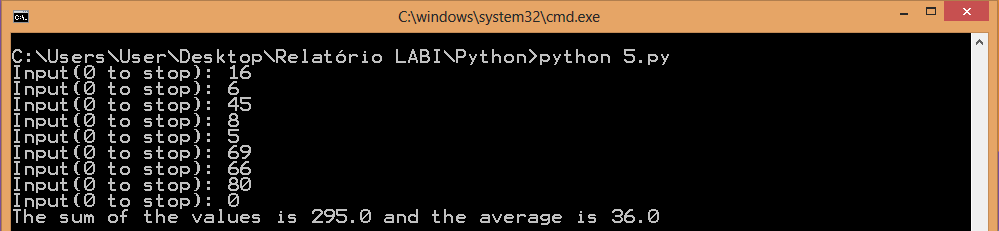
\includegraphics[width=\textwidth]{cmd_5.png}
 \caption{Execução do Exercício 5}
 \label{cmd5}
\end{figure}


O código de Java pode ser consultdo na \autoref{java.5} e o código de Python na \autoref{python.5}.
\\[5pt]
O facto de, em Python, a indentação influenciar o funcionamento do código, faz com que o este se torne mais legível, uma vez que o utilizador é forçado a utilizar uma indentação fixa.
\\[5pt]
A regra "\gls{Beautiful is better than ugly}." está novamente presente.

\clearpage



\section{Exercício 6}
\label{exercicio6}

Escreva um programa que implemente o jogo “Adivinha o número!”.


Neste jogo, o programa deve escolher um número aleatório no intervalo [0; 100], dando depois a possibilidade de o utilizador ir tentando descobrir o número escolhido. 

Para cada tentativa, o programa deve indicar se o número escolhido é maior, menor ou igual à tentativa feita. 

O jogo termina quando o número correcto for indicado , sendo a pontuação, do jogador o número de tentativas feito (portanto o valor 1 será pontuação máxima).



\begin{figure}[ht]
 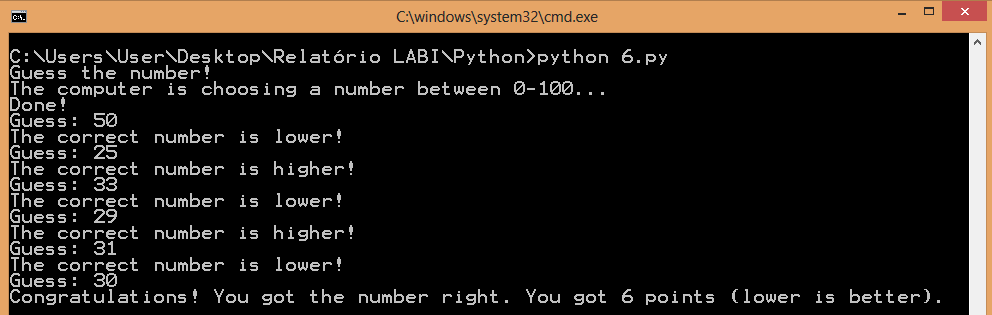
\includegraphics[width=\textwidth]{cmd_6.png}
 \caption{Execução do Exercício 6}
 \label{cmd6}
\end{figure}


O código de Java pode ser consultdo na \autoref{java.6} e o código de Python na \autoref{python.6}.

Apesar de, em Java, também existir um comando que gera um número aleatório, este é muito mais simples e perceptível em Pyton.
\begin{description}
    \item \textbf{Java} - \fbox{n=(int)(Math.random()*(100+1));}
    \item \textbf{Python} - \fbox{num = randint(1,100)}
\end{description}

Este aspecto segue a regra "\gls{Simple is better than complex}."

\clearpage

\section{Exercício 7}
\label{exercicio7}
Crie um programa que copie um ficheiro de texto para outro. Os nomes dos dois ficheiros envolvidos devem ser dados como argumentos na linha de comandos. Assim a execução do programa com os argumentos Texto1.txt Texto2.txt deve criar um ficheiro Texto2.txt com um conteúdo igual ao do ficheiro Texto1.txt.


Nota: Tente fazer com que o programa tenha alguma robustez, não só detectando a existência do ficheiro original (apresentando uma mensagem de erro quando este não existe), como também a possível existência do ficheiro destino (neste caso fará sentido perguntar ao utilizador se de facto deseja destruir esse ficheiro). Deve também verificar se sobre os ficheiros se podem realizar as operações de leitura e escrita, e se algum deles é um directório (caso em que deve ser apresentada uma mensagem de erro).


\begin{figure}[ht]
 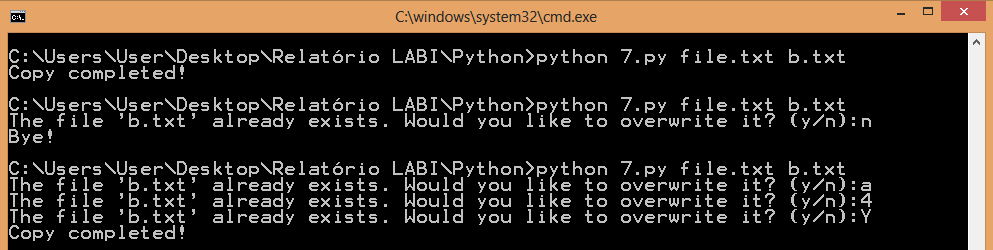
\includegraphics[width=\textwidth]{cmd_7.png}
 \caption{Execução do Exercício 7}
 \label{cmd7}
\end{figure}


O código de Java pode ser consultdo na \autoref{java.7} e o código de Python na \autoref{python.7}.

Neste exercício observam-se grandes diferenças no que toca a manipulação de ficheiros.
\\[5pt]
Criação de uma variável do tipo File:
\begin{description}
    \item \textbf{Java} - \fbox{File fin = new File(args[0]);}
    \item \textbf{Python} - \fbox{file\_in = open(name\_in, "r")}
\end{description}
Como se pode constatar, a principal diferença é o facto de, em Python, se poder definir se se quer utilizar esse ficheiro para ler, escrever ou ambos.
\clearpage
Em Java é necessário criar scanners associados a um ficheiro para os poder ler, e printwriters para escrever em ficheiros. Em Python, abrir, ler e escrever em ficheiros pode ser feito através de comandos muito mais simples, sem haver a necessidade de criar scanners ou printwriters.
\\[5pt]
Ler de um ficheiro:
\begin{description}
    \item \textbf{Java} - \fbox{String a = sc.nextLine()}
    \item \textbf{Python} - \fbox{line q= file\_in.readline()}
\end{description}
Escrever num ficheiro:
\begin{description}
    \item \textbf{Java} - \fbox{PrintWriter pw = new PrintWriter(fout); pw.println(a);}
    \item \textbf{Python} - \fbox{file\_out.write(line)}
\end{description}
\clearpage
\section{Análise Geral \footnotesize Adaptado de Udemy\cite{Udemy}}
\subsection{Tipos estáticos vs. tipos dinâmicas}
\begin{enumerate}
    \item \textbf{Java} - As variáveis em Java têm de ter o seu tipo definido desde a sua declaração, não podendo ser mudado ao longo do programa.
    \item \textbf{Python} - As variáveis têm tipos dinâmicos, isto é, não é necessário definir um tipo de variável e este pode mudar ao longo do programa.
\end{enumerate}
Variáveis com tipos dinâmicos torna a tarefa de programar mais fácil, principalmente para programadores principiantes. Porém, tipos estáticos reduzem o risco de ocorrência de erros, pois, em Python, existe o risco de, ao cometer erros de ortografia, declarar uma variável nova, o que irá influenciar o funcionamento do programa.
\subsection{Chavetas vs. Indentação}
\begin{enumerate}
    \item \textbf{Java} - Utiliza chavetas para definir os blocos de código.
    \item \textbf{Python} - Utiliza a indentação para definir os blocos de código.
\end{enumerate}
Como foi referido no \autoref{exercicio5}, o facto do Python forçar o utilizador a usar indentação no seu código torna-o mais legível e melhor esteticamente.("\gls{Beautiful is better than ugly}."/"\gls{Readability counts}.")
\clearpage
\subsection{Portabilidade vs Velocidade}
\begin{enumerate}
    \item \textbf{Java} - A maioria dos sistemas suporta a execução de aplicações em Java. Porém, num ambiente virtual, é mais lento que Python.
    \item \textbf{Python} - Para executar códigos em Python é necessário o sistema ter um compilador que converta o código em Python para outro código que o sistema consiga interpretar. Apesar disto, a sua velocidade de execução é bastante alta
\end{enumerate}


Mais uma vez, "\gls{Explicit is better than implicit}.", como é mostrado na funcionalidade de escrever ou ler através das funções acima. Em Java, com a utilização de um scanner, não é tão evidente que se está a efectuar, por exemplo, uma leitura.



\chapter{Conclusão}
\label{conclusion}


Depois de comparar os códigos dos dois exercícios, concluíu-se que ao escolher uma implementação em Python, o código resultante será mais legível e conciso.
\\
Python é mais acessível a programadores principiantes, uma vez que as variáveis possuem tipos dinâmicos e as funções existentes são explícitas e intuitivas. 
\\
Também tem a vantagem de ser rápido a executar. A legibilidade e simplicidade do código é a principal característica que distingue esta liguagem das outras.

\addcontentsline{toc}{chapter}{Glossário}
\renewcommand*{\glossaryname}{Glossário}

\printglossaries

\bibliography{references}

\appendix
\chapter{Exercício 1}
\section{Java}
\label{java.1}
\footnotesize
\lstinputlisting[language=Java]{Ex1.java}

\section{Python}
\label{python.1}
\lstinputlisting[language=Python]{1.py}

\chapter{Exercício 2}
\section{Java}
\label{java.2}
\lstinputlisting[language=Java]{ex2.java}

\section{Python}
\label{python.2}
\lstinputlisting[language=Python]{2.py}

\chapter{Exercício 3}
\section{Java}
\label{java.3}
\lstinputlisting[language=Java]{ex3.java}

\section{Python}
\label{python.3}
\lstinputlisting[language=Python]{3.py}

\chapter{Exercício 4}
\section{Java}
\label{java.4}
\lstinputlisting[language=Java]{ex4.java}

\section{Python}
\label{python.4}
\lstinputlisting[language=Python]{4.py}

\chapter{Exercício 5}
\section{Java}
\label{java.5}
\lstinputlisting[language=Java]{Ex5.java}


\section{Python}
\label{python.5}
\lstinputlisting[language=Python]{5.py}

\chapter{Exercício 6}
\section{Java}
\label{java.6}
\lstinputlisting[language=Java]{Ex6.java}

\section{Python}
\label{python.6}
\lstinputlisting[language=Python]{6.py}

\chapter{Exercício 7}
\section{Java}
\label{java.7}
\lstinputlisting[language=Java]{Ex7.java}

\section{Python}
\label{python.7}
\lstinputlisting[language=Python]{7.py}

\end{document}
